\begin{figure}[htbp]
  \centering
  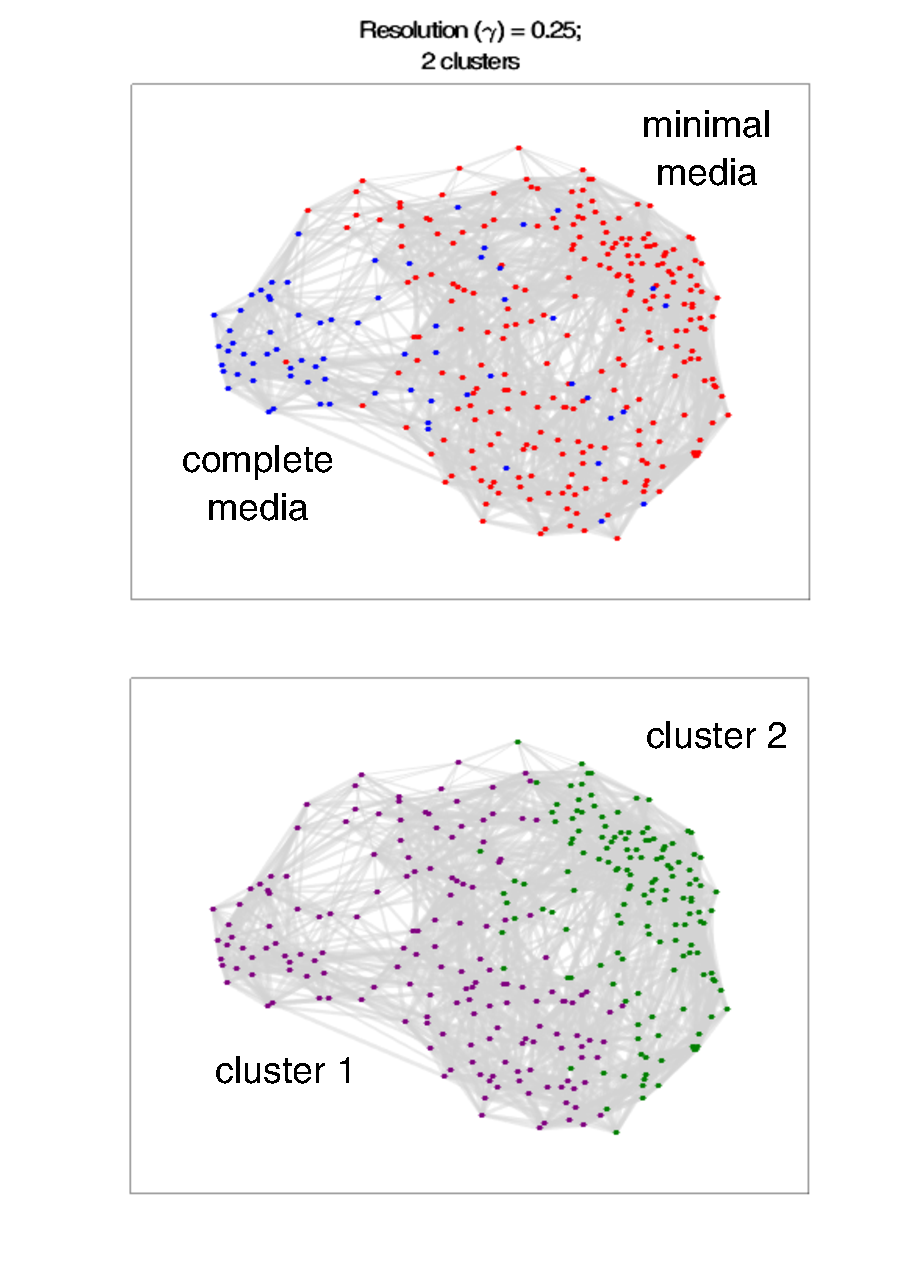
\includegraphics[width=0.5\textwidth]{10m_EffectofMediaClusters}
  \caption{Graph-based clustering partitions a geometric graph defined by pairwise cosine distances between \textit{catch22} vectors close to labels defined by media.}
  \label{fig:EffectofMediaClusters}
\end{figure}

Indeed, I found that the method was able to distinguish time series generated in my project from time series obtained by \textcite{baumgartnerFlavinbasedMetabolicCycles2018} (figure \ref{fig:DistanceMatrixBaumgartner}, table \ref{tab:ClusterBaumgartner})
However, this ability to distinguish the data sources may have been because the data from different sources were processed in different ways.

\begin{figure}[htbp]
  \centering
  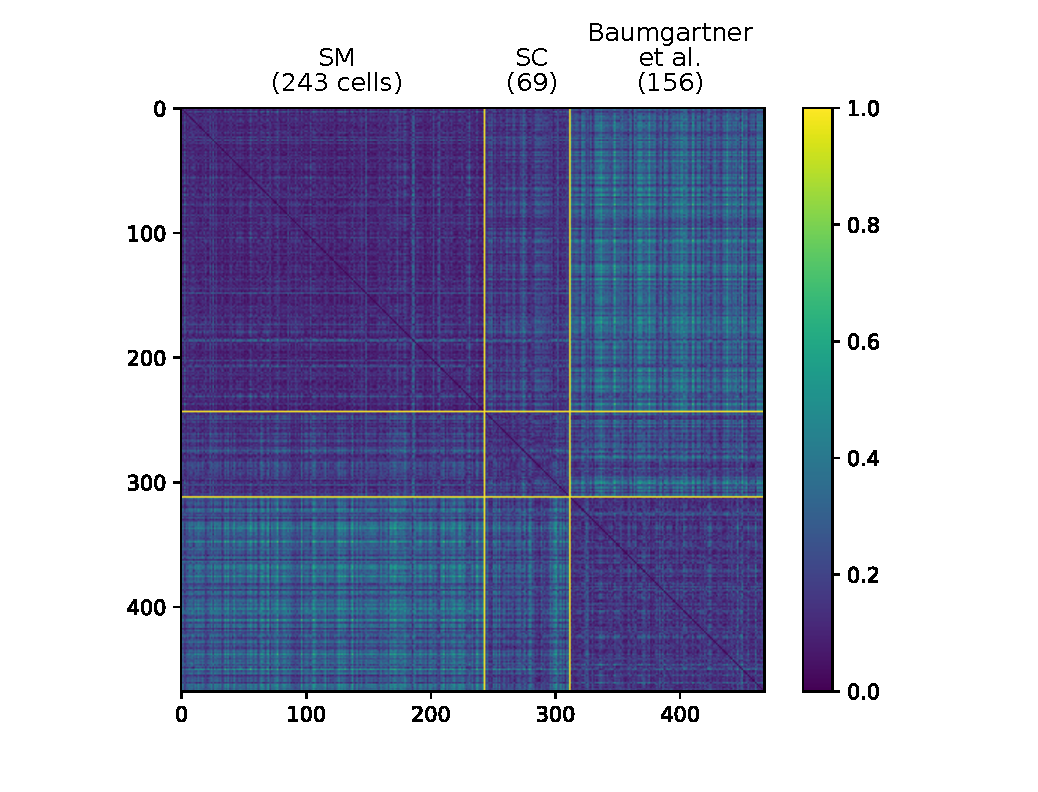
\includegraphics[width=0.6\textwidth]{10m_DistanceMatrixBaumgartner}
  \caption{Graph-based clustering was able to partition minimal media time series, complete media time series, and time series from \textcite{baumgartnerFlavinbasedMetabolicCycles2018}.
    This distance matrix is based on cosine distances between \textit{catch22} feature vectors for pairs of time series.  Distances between 0 and 1 (legend, right) are represented as colours.}
  \label{fig:DistanceMatrixBaumgartner}
\end{figure}

\begin{table}[htbp]
  \centering
  \begin{tabular}[h]{rrrr}
    & SM & SC & Baumgartner et al.\\
    Cluster 1 & 1 & 11 & 141\\
    Cluster 2 & 63 & 28 & 6\\
    Cluster 3 & 56 & 22 & 8\\
    Cluster 4 & 79 & 4 & 0\\
    Cluster 5 & 44 & 4 & 1
  \end{tabular}
  \caption{Graph-based clustering is able to partition minimal media time series, complete media time series, and time series from \textcite{baumgartnerFlavinbasedMetabolicCycles2018}.  Table shows one graph partition returned by the general Louvain algorithm.  The graph was constructed according to section [METHODS: HCTSA].  In this case, the default value for the resolution parameter was used.}
  \label{tab:ClusterBaumgartner}
\end{table}
% Rand index?

\subsection{Linear techniques}
\label{subsec:analysis-clustering-pca}

(Space for PCA and PCA-initiated t-SNE that I did while doing the UMAP project)
